\chapter{Numerical Simulation of Unsteady Laminar Flow}
\section{Problem Description}
\subsection{Governing Equations} % homogenous fluid region, and porous region
\subsection{Boundary Conditions} % Including interface between the homogeneous fluid and porous medium regions


\section{Numerical Methods}
\subsection{Discrete Methods of Time and Space}
\subsection{Solver} % SIMPLE
\subsection{Mesh Generation and Independence Analysis}
The flow domain is divided into three blocks, as described in Figure \ref{fig: grid}. The grid size is shown in Table \ref{tab: grid}. The Reynolds number and the Darcy number are 100 and 0.0001 separately.

\begin{figure}
	\centering
	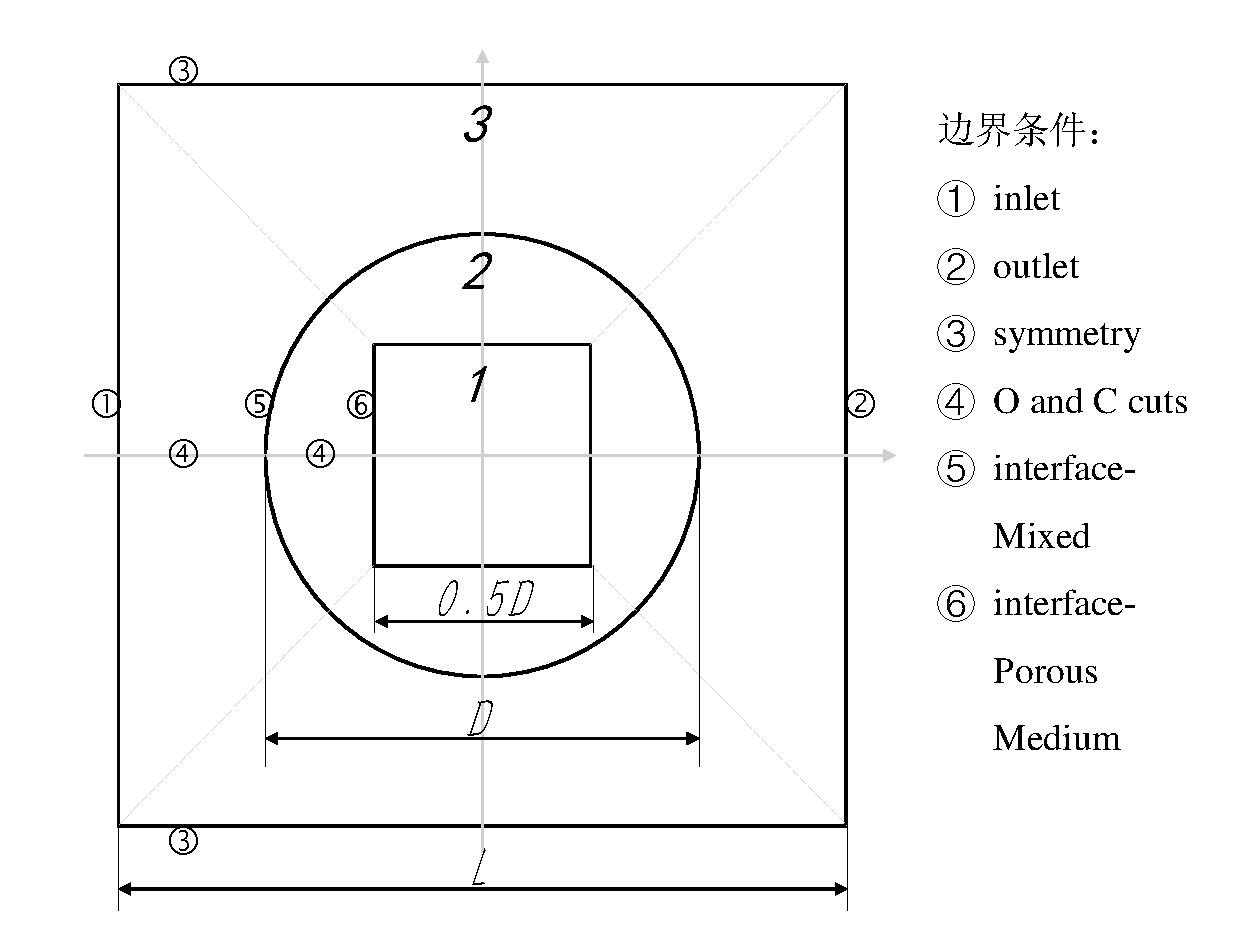
\includegraphics[scale=.6]{../diagrams/grid}
	\caption{The partition of grid blocks.}\label{fig: grid}
\end{figure}
\begin{table}[h]
	\centering
	\caption{My caption}
	\label{tab: grid}
	\begin{tabular}{@{}ccccc@{}}
		\toprule
		\multicolumn{2}{c}{Blocks}  & Block 1  & Block 2   & Block 3    \\ \midrule
		\multirow{4}{*}{Grid size} 
		& Case 1 & 40 $\times$ 40 & 160 $\times$ 25 & 160 $\times$ 140 \\
		& Case 2 & 60 $\times$ 60 & 240 $\times$ 30 & 240 $\times$ 170 \\
		& Case 3 & 80 $\times$ 80 & 320 $\times$ 40 & 320 $\times$ 200 \\
		& Case 4 & 100 $\times$ 100 & 400 $\times$ 50 & 400 $\times$ 230 \\
		\bottomrule
	\end{tabular}
\end{table}


\section{Summary}
